\documentclass[10 pt]{article}
\usepackage{graphicx}
\pagestyle{plain}
\usepackage[OT4]{polski}
\usepackage[utf8]{inputenc}
\title{Sprawozdzanie 2 \\ \emph{ \textbf{ Sortowanie 2}}}
\author{Paweł Żurek 200404}
\date{17.03.2014}
\begin{document}
\tableofcontents
\maketitle
\section{Wstep}
\textbf{Do posortowania zbioru losowo wygenerowanych elementów użyłem : }
\begin{itemize}
\item Qucik Sort ( Sortowanie Szybkie )
\item Merge Sort ( Sortowanie przez scalanie )
\item Heap Sort ( Sortowanie przez kopcowanie)
\end{itemize}
\textbf{Sortowanie zostało przeprowadzone dla następującej ilości elementów : }
\begin{itemize}
\item 10
\item 100
\item 1000
\item 10000
\item 100000
\item 1000000
\end{itemize}
\textbf{Sortowanie zostało przeprowadzone dla następująco wypełnionych tablic : }
\begin{itemize}
\item Posortowanych rosnąco
\item Posortowanych malejąco
\item Wypełnionych losowo
\end{itemize}

\section{Wyniki}

\paragraph{Dane zebrane w formie tabeli ( tylko wartości uśrednione ) : \\}
\begin{center}
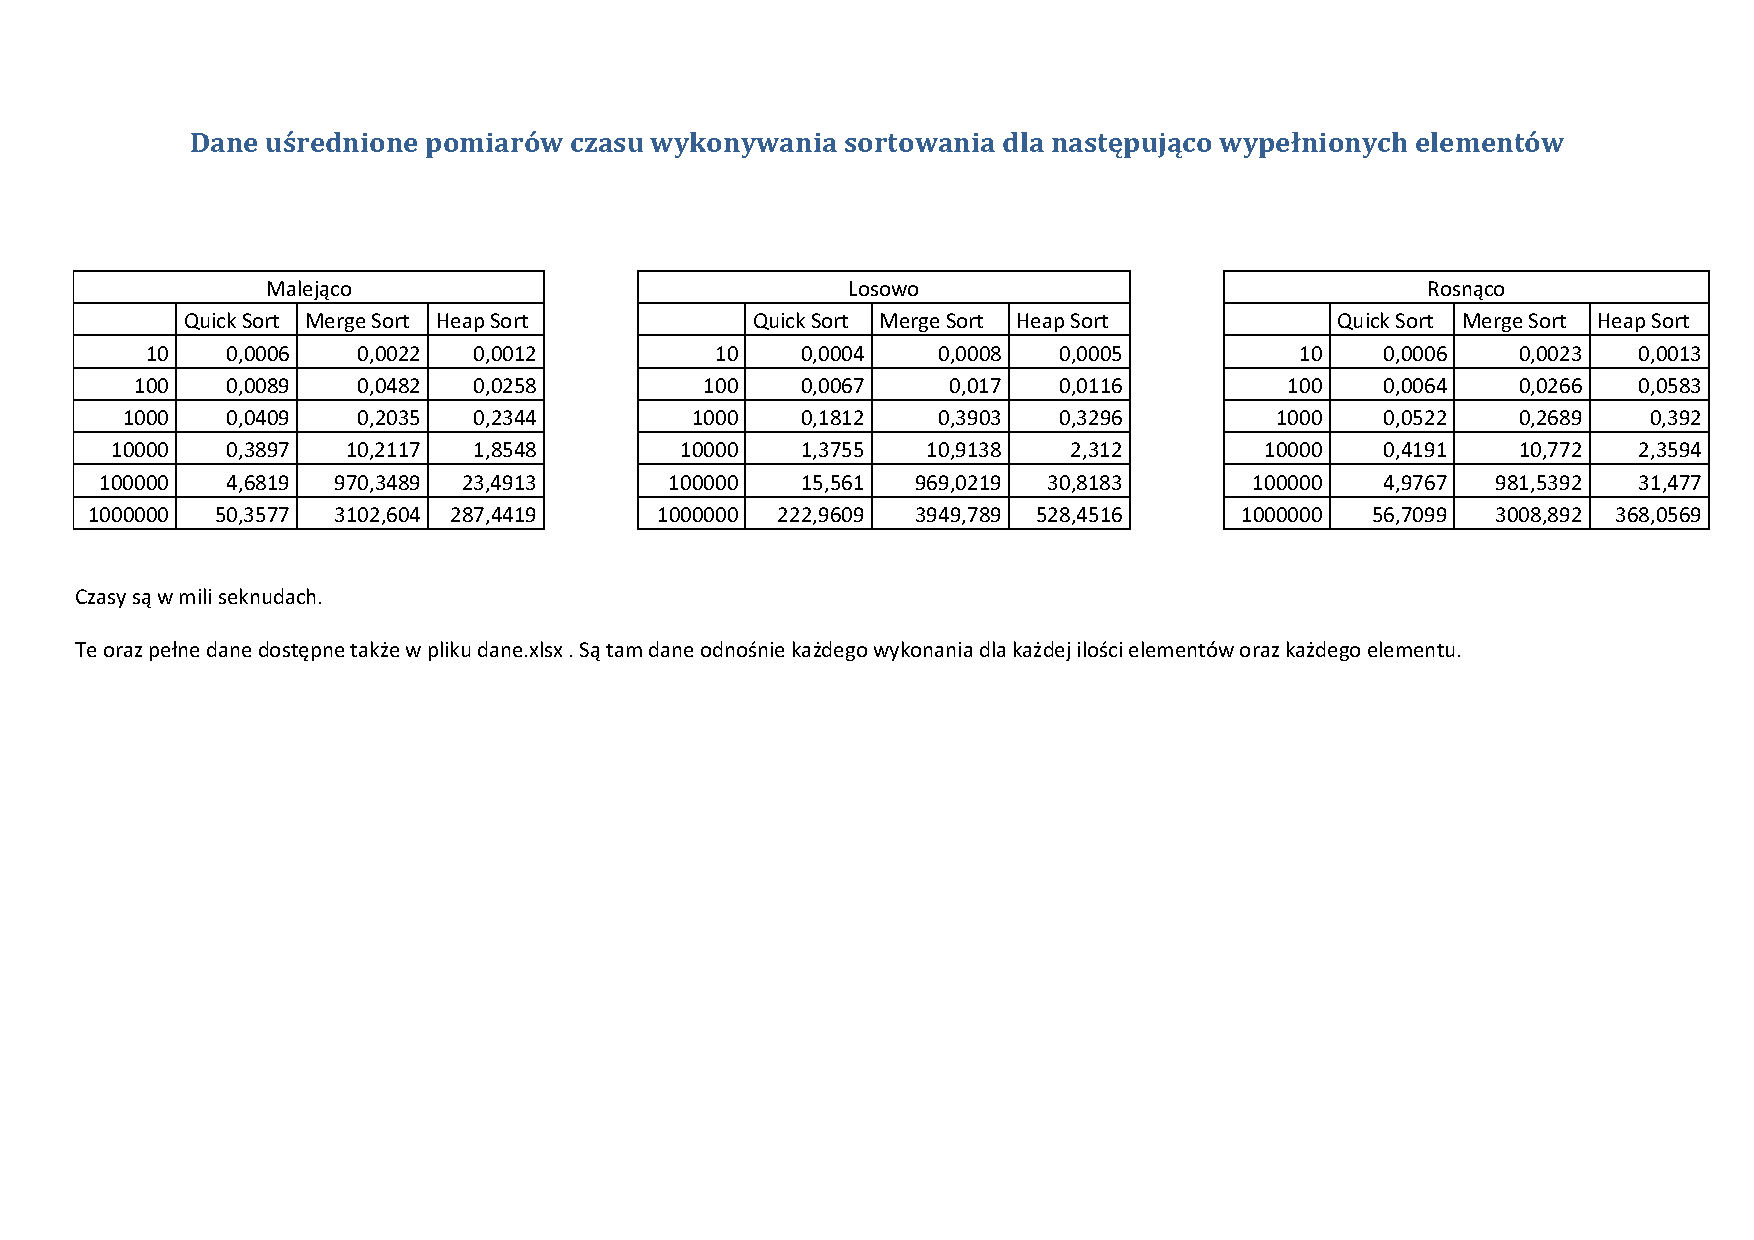
\includegraphics[scale=0.5]{DaneUsrednione.pdf}
\end{center}
\newpage
\paragraph{Dane wyświetlone za pomoca wykresu ( wykres dostępny osobno w pliku Wykres1.pdf) }
\begin{center}
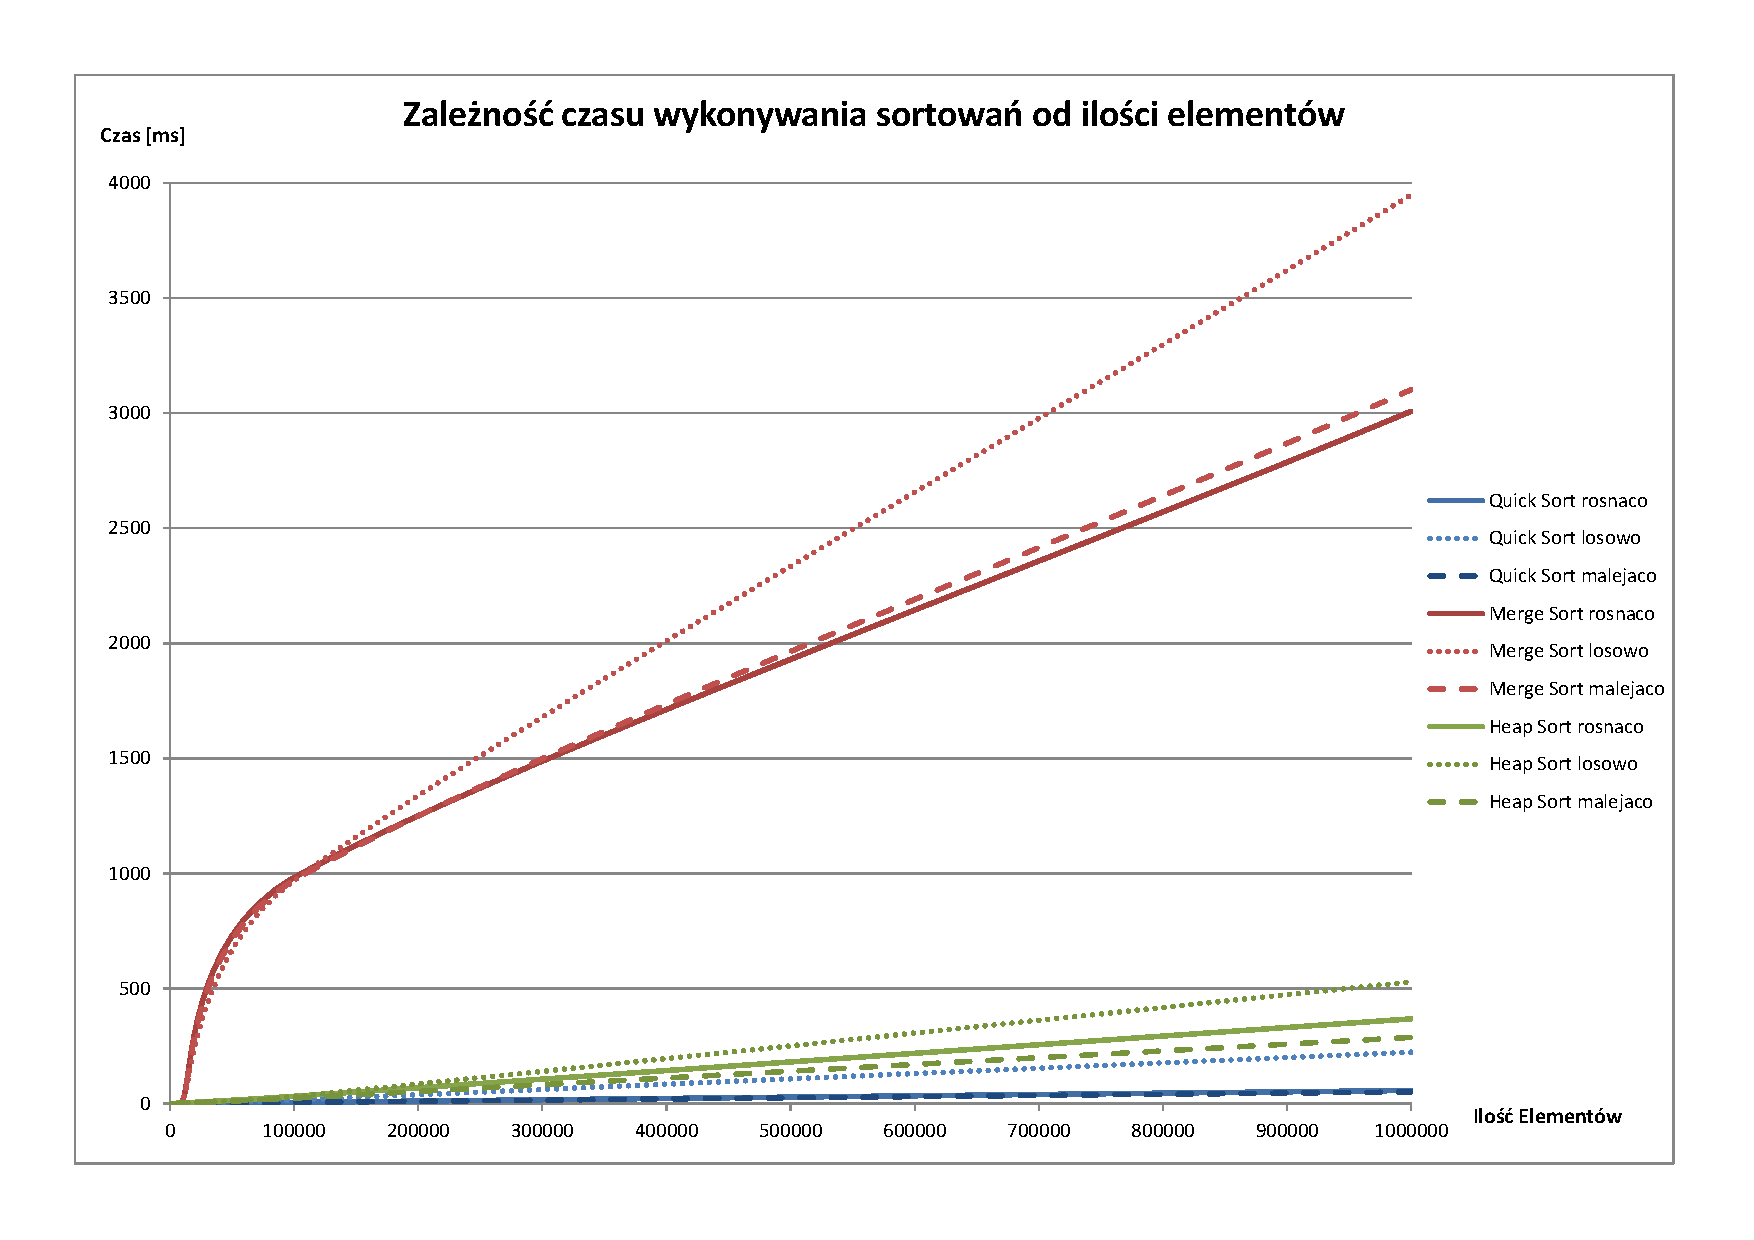
\includegraphics[scale=0.4]{Wykres1.pdf}
\end{center}

\paragraph{Wykres przybliżony ( wykres dostępny osobno w pliku Wykres2.pdf) }
\begin{center}
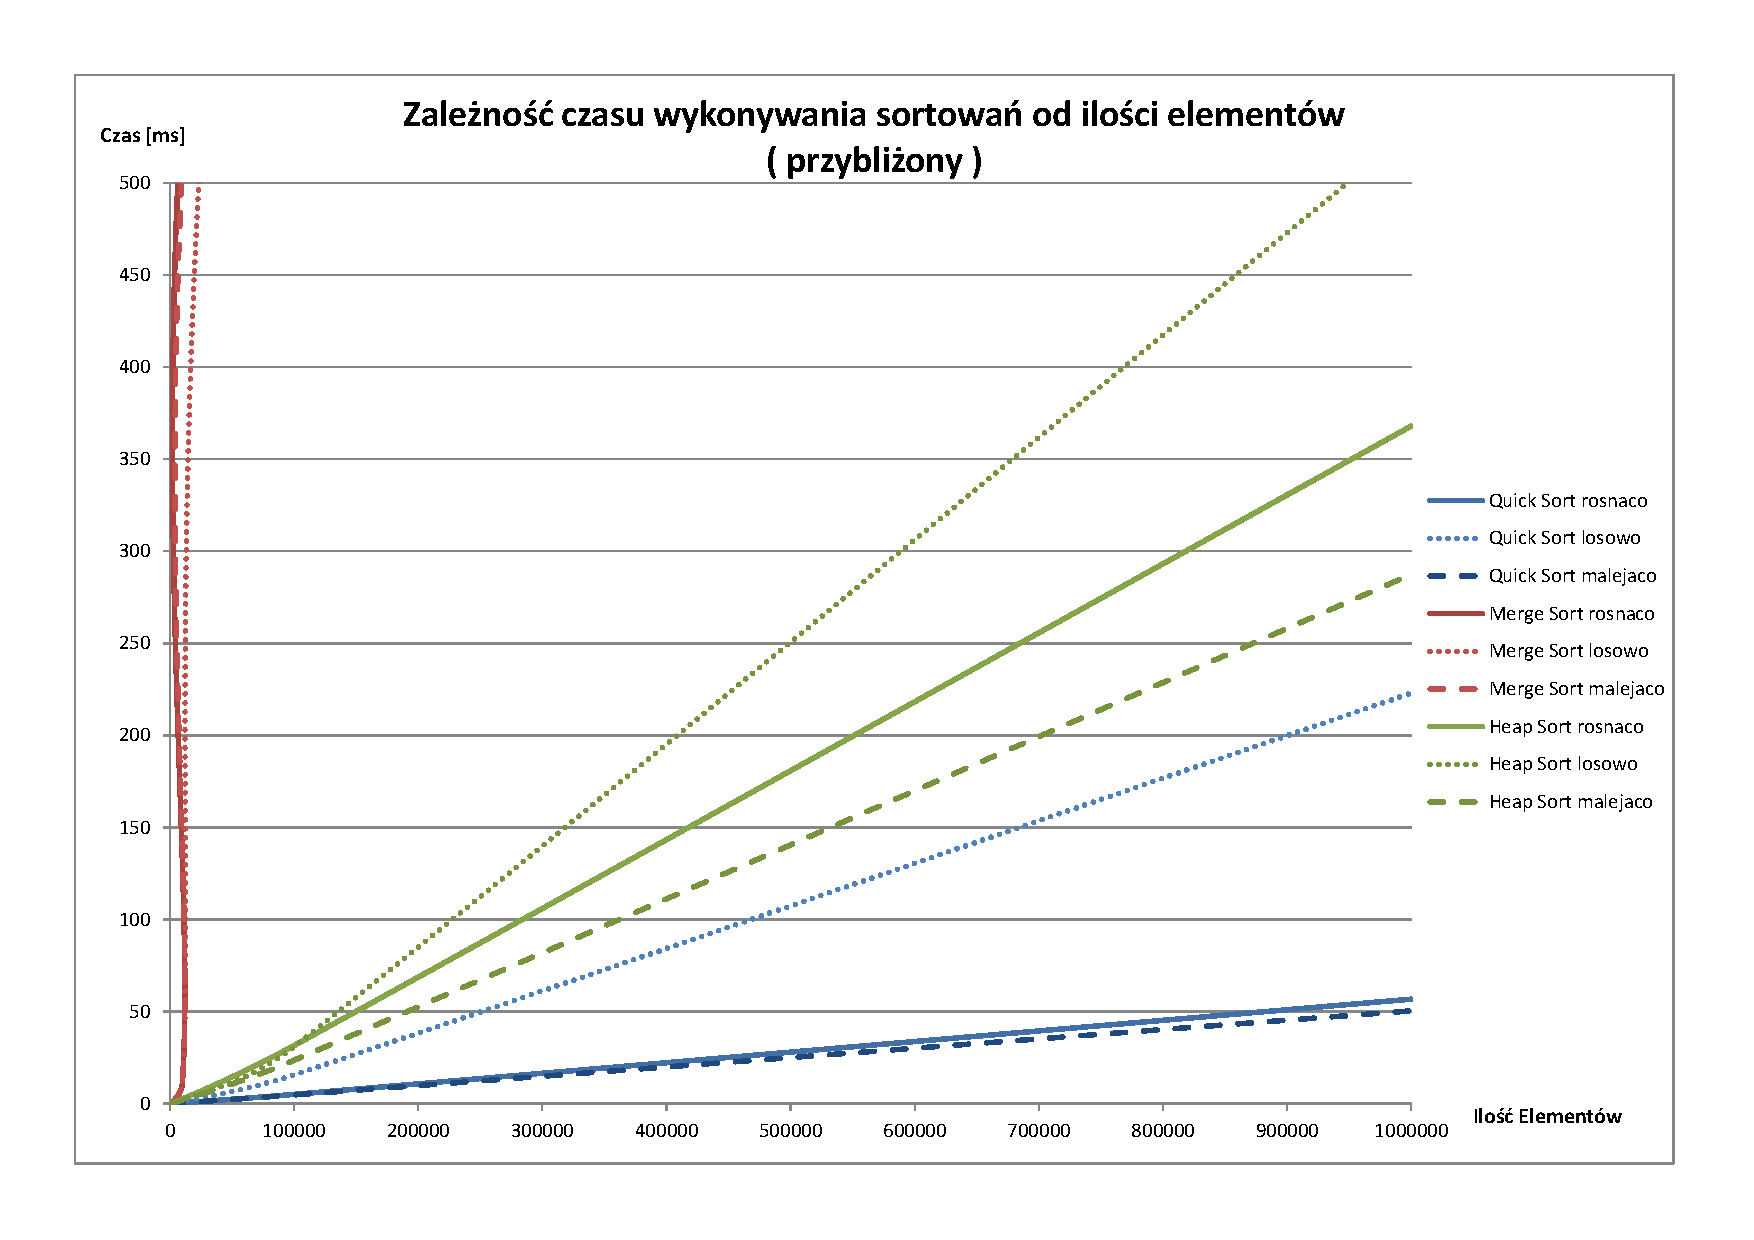
\includegraphics[scale=0.4]{Wykres2.pdf}
\end{center}

\section{Wnioski:}
\begin{itemize}
\item Dla każdego algorytmu, posortowanie elementów wypełnionych losowo trwało najdłużej
\item Dla elementów posortowanych rosnąco i malejąco różnice w czasie są na tyle małe, iż można uznać, że
zajmują podobną ilość czasu dla każdego algorytmu. Aczolwiek z tych trzech, Merge Sort jest jedyną metodą,
której posortowanie elementów posortowanych malejąco zajęło więcej czasu niż elementów posortowanych
rosnąco
\item Posortowanie elementów wypełnionych losowo dla metody Quick Sort ( mimo tego, że dla tej metody
najwolniejsze ) i tak okazało się szybsze niż inne metody ( nawet z elementami posortowanymi )
\item Posortowanie elementów wstępnie posortowanych okazało się szybsze. Dzieje się tak, ponieważ większość
algorytmów zamienia elementy po porównaniu elementów. Jeśli zbiór już jest posortowany, jest po prostu
mniej operacji zamiany wartości elementów. To znacznie przyśpiesza wykonywanie algorytmu. Dla
algorytmu Quick Sort więcej niż 4 razy
\item Na wykresie numer 2, przybliżonym, widać dziwne zachowanie lini Merge Sort. Jest to spowodowane małą
ilością punktów pomiarowych. Program wypełnia sam miejsca gdzie nie ma tych punktów przwidując ich
położenie, co często nie jest poprawnie robione
\item Sortowanie zostało wykonane za każdym razem 10 razy. Za każdym razem czas wykonywania różni się, co
widać w pliku z danymi. Prawdopobnie jest to spowodowane tym, iż za każdym razem procesor wykonuje
inne obliczenia w tle podczas wykonywania programu

\end{itemize}
Dokumentacja program dostępna w pliku pdf o nazwie ''Dokumentacja'' (zapisana w \LaTeX u) oraz w DoxyGen'ie (dostępna w pliku : dox/html/index.html)

\end{document}